We investigated two practical architectures for the co-located integrated information and energy receiver. Both designs are equipped with individual ID and EH receivers. The former is a conventional baseband demodulator while the latter can be realized with the proposed rectifier structure in Section \ref{sec:rectenna-design}.



\subsection{Time Switching}\label{sec:time-switching}
A \textit{Time Switching (TS)} receiver (Figure \ref{fig:ts-receiver}) operates as either an information decoder or an energy harvester at a certain time. In the design, the transmitter divides the transmission block into orthogonal power and data slots with length ratio $\alpha $ and $1 - \alpha $ respectively, then optimizes the waveform for WPT or WIT individually. Also, the receiver periodically switches between ID and EH receivers in the corresponding slots. We assume perfect synchronization between transmitter and receiver for mode control. It can achieve different rate-energy tradeoffs by adjusting the slot length ratio $\alpha $ jointly with the transmit signals. As the input power range for information and power receivers are typically different, TS can be combined with a "near-far" scheduling \cite{Zhang2013} to benefit the system efficiency.

\begin{figure}
  \centering
    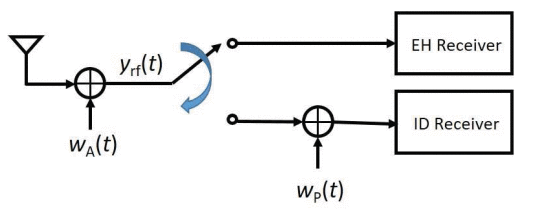
\includegraphics[width=\textwidth]{ts_receiver}
  \caption{Structure of time switching receiver \cite{Clerckx2019}}
  \label{fig:ts-receiver}
\end{figure}



\subsection{Power Splitting}\label{sec:power-splitting}
In a \textit{Power Splitting (PS)} receiver (Figure \ref{fig:ps-receiver}), we introduce a PS ratio $\rho $ to split the received signal into separate power stream (with proportion $\rho $) and information stream (with proportion $1 - \rho $). At the transmitter, the signal is jointly optimized for information and power transmission according to CSIT. With the assumption of perfect matching, the EH and ID receivers are with input voltage signals $\sqrt {\rho {R_{{\text{ant}}}}} y(t)$ and $\sqrt {(1 - \rho ){R_{{\text{ant}}}}} y(t)$ respectively. Varying the PS ratio $\rho $ and the transmit signals leads to different rate-energy points. It is argued in \cite{Zhang2013} that the PS scheme is optimal for ideal RF-to-baseband signal conversion with negligible processing noise, but the condition is hard to meet in practice.

\begin{figure}
  \centering
    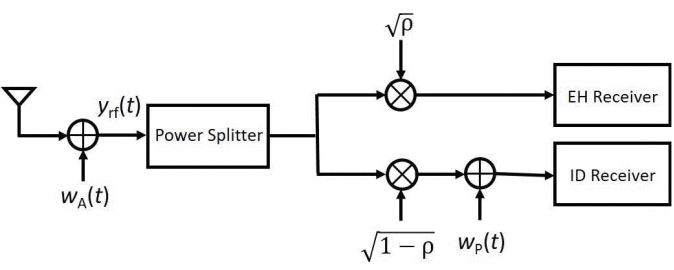
\includegraphics[width=\textwidth]{ps_receiver}
  \caption{Structure of power splitting receiver \cite{Clerckx2019}}
  \label{fig:ps-receiver}
\end{figure} 